\documentclass[12pt,letterpaper]{article}

\usepackage{fancyhdr}
\pagestyle{fancy}
\fancyhf{}
\rhead{Vaja 9}
\lhead{ORS}
\setlength{\headheight}{16pt}

\usepackage[utf8]{inputenc}
\usepackage[slovene]{babel}
\usepackage[colorlinks = true, urlcolor = blue]{hyperref}

\usepackage{xcolor}
\usepackage{listings}
\usepackage{graphicx}
\graphicspath{{./images/}}
\definecolor{mGreen}{rgb}{0,0.6,0}
\definecolor{mGray}{rgb}{0.5,0.5,0.5}
\definecolor{mPurple}{rgb}{0.58,0,0.82}
\definecolor{backgroundColour}{rgb}{1,1,1}

\lstdefinestyle{CStyle}{
    backgroundcolor=\color{backgroundColour},
    commentstyle=\color{mGreen},
    keywordstyle=\color{magenta},
    numberstyle=\tiny\color{mGray},
    stringstyle=\color{mPurple},
    basicstyle=\footnotesize,
    breakatwhitespace=false,
    breaklines=true,
    captionpos=b,
    keepspaces=true,
    numbers=left,
    numbersep=5pt,
    showspaces=false,
    showstringspaces=false,
    showtabs=false,
    tabsize=2,
    language=C,
    frame=none
}

\begin{document}

\begin{center}
    \textbf{\Large Neposreden dostop do pomnilnika (DMA) v STM32F4}
\end{center}

Na zadnji letošnji vaji se bomo spoznali z napravo, ki omogoča prenos podatkov med perifernimi napravami in pomnilnikom brez posredovanja centralne procesne enote. Te naprave poznamo pod kratico DMA, ki izhaja iz angleškega izraza direct memory access. Na predavanjih ste spoznali, da obstaja več različnih implementacij neposrednega dostopa do pomnilnika, za potrebe vaj bomo spoznali način izvedbe DMA prenosov v krimilnikih družine STM32F4.

Primer uporabe DMA krmilnika je sprejem večjega števila bajtov z up naprave USART1. Pri klasičnem pristopu, brez DMA krmilnika, bi to storili tako, da bi krmilnik sprejel vsak bajt posebej (s prekinitvami ali brez) in ga shranil na svoje mesto v polju ustrezne velikosti. Z uporabo DMA krmilnika lahko isto nalogo opravimo brez posredovanja CPE. S tem CPE razbremenimo izvajanja enostavnih pomnilniških operacij, pri katerih so same operacije trivialne, CPE pa večino časa zgolj čaka, da so podatki na voljo. V tem času lahko CPE izvaja pomembnejša opravila oziroma ``počiva'', saj CPE med svojim običajnim delovanjem porabi precej električne energije.


\section*{DMA streami in kanali}

Mikrokrmilnik STM32F407 ima dva DMA krmilnika, oba lahko hkrati upravljata z osmimi tokovi podatkov (angl. stream). Podatkovni tokovi so označeni z oznakami Stream 0 do Stream 7. Podatkovni tok je lahko na primer zgoraj omenjen primer shranjevanja podatkov iz naprave USART1 v pomnilnik. Za vsakega izmed osmih podatkovnih tokov ima DMA krmilnik nabor osmih možnosti, ki določajo kaj in v kateri smeri se bo prenašalo. Te možnosti imenujemo kanali (angl. Channels). Sliki \ref{dma1_stream} in \ref{dma2_stream} prikazujeta tabeli kanalov za posamezne podatkovne tokove. Stream 3 naprave DMA1 tako lahko neposredno v pomnilnik zapisuje podatke, ki jih prejme naprava SPI2 ali naprava UART7. Lahko pa tudi neposredno iz pomnilnika pošilja podatke napravi USART3.

\begin{figure}[ht!]
  \centering
  \caption{Streami in kanali DMA1.}
  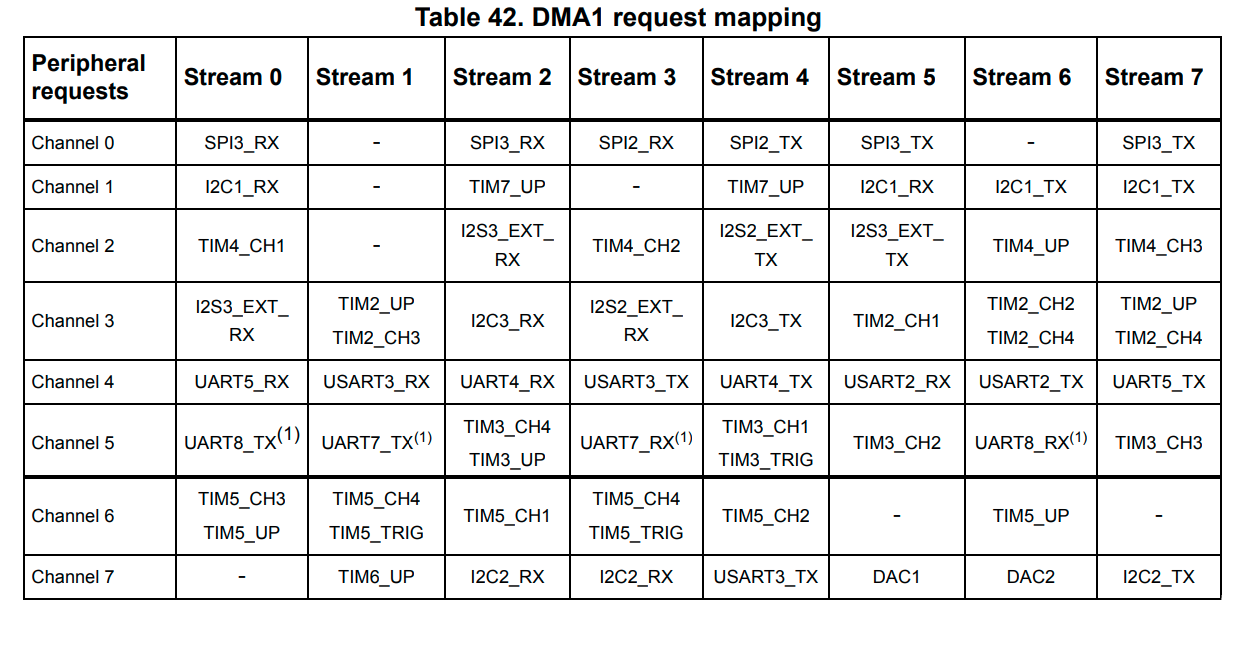
\includegraphics[width=330px]{images/vaja9/DMA1.png}
  \label{dma1_stream}
\end{figure}

\begin{figure}[ht!]
  \centering
  \caption{Streami in kanali DMA2.}
  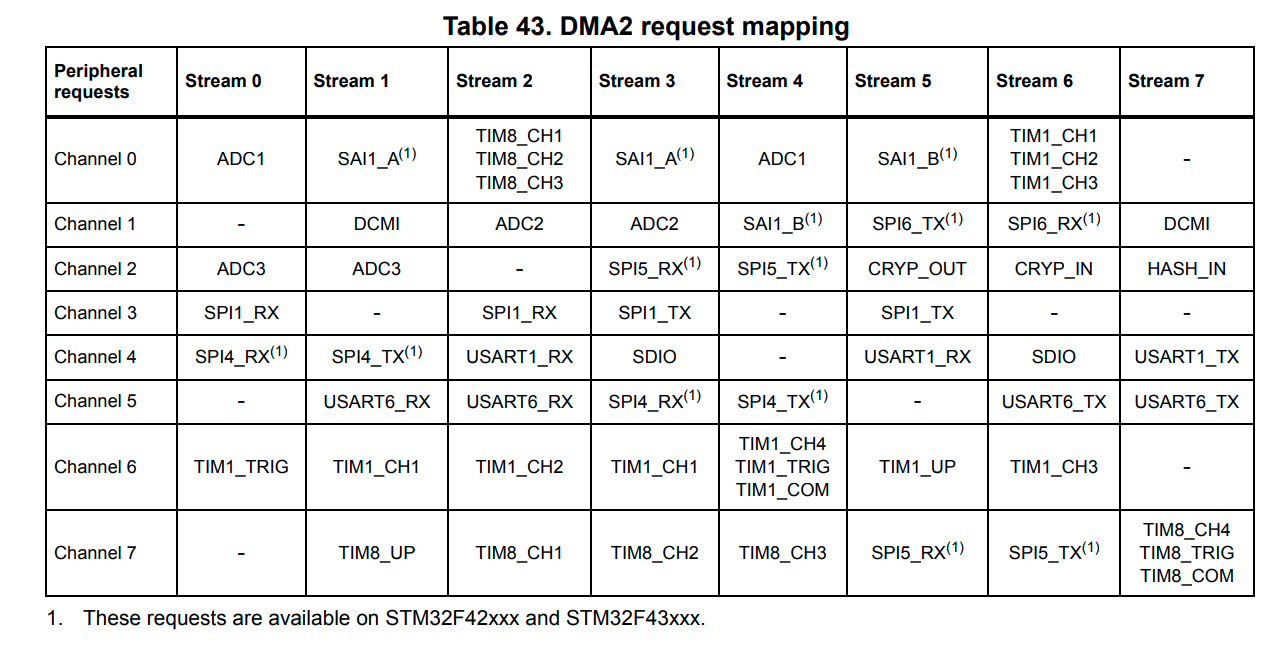
\includegraphics[width=330px]{images/vaja9/DMA2.png}
  \label{dma2_stream}
\end{figure}

Vsaka DMA naprava upravlja z do osmimi podatkovnimi tokovi naenkrat. V danem trenutku je aktiven zgolj en podatkovni tok, ostali pa takrat čakajo. Izbiranje aktivnega podatkovnega toka izvaja arbiter na podlagi prioritete posameznega toka. Prioriteto podatkovnega toka določimo programsko, izbiramo lahko med štirimi nivoji prioritete: nizka, srednja, visoka in zelo visoka.


\section*{Nastavitve DMA prenosa}

DMA prenosu moramo določiti več lastnosti. Prva je smer prenosa, ki je lahko \textit{od periferne naprave do pomnilnika} (angl. peripheral to memory), \textit{ od pomnilnika do periferne naprave} (angl. memory to peripheral) ali pa \textit{od pomnilnika do pomnilnika} (angl. memory to memory). Slednjega je sposobna samo naprava DMA2. To lahko uporabimo, ko želimo na primer prekopirati vsebino daljšega polja na drug naslov.

Poleg smeri moramo določiti tudi izvorni (angl. source) in ciljni oz. ponorni (angl. destination) naslov DMA prenosa. V primeru prenosa od periferne naprave do pomnilnika je izvorni naslov register naprave, ciljni naslov pa naslov spremenljivke ali polja v pomnilniku. V primeru obratne smeri prenosa je ravno obratno. Določiti moramo tudi ali se izvorni oziroma ciljni naslov med prenosom povečujeta (angl. increment). Če pošiljamo podatke iz polja ali podatke sprejemamo v polje je namreč potrebno izvorni ali ciljni naslov po vsakem prenosu povečati. V nasprotnem primeru bi vsak podatek zapisali na isto mesto. Prikaz povečevanja ciljnega naslova je prikazan na sliki \ref{inkrementnaslovov}.

\begin{figure}[ht!]
  \centering
  \caption{Povečevanje ciljnega naslov pri DMA prenosu.}
  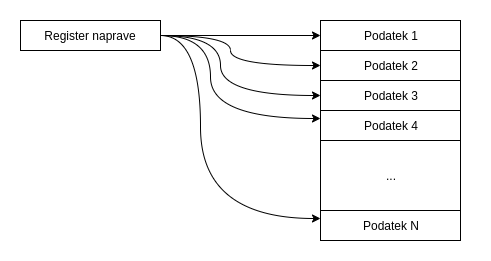
\includegraphics[width=330px]{images/vaja9/inkrement_prenos.png}
  \label{inkrementnaslovov}
\end{figure}

Določiti je potrebno tudi dolžino prenosa (označeno s črko N na sliki \ref{inkrementnaslovov}) in velikost posameznega podatka. Podatek je lahko bajt (angl. byte), dva bajta (angl. half-word) ali štiri bajti (angl. word).

Izbiramo lahko med dvema tipoma prenosa: normalnim in krožnim. Pri prvem se izvrši prenos N podatkov, nato pa se DMA prenos konča. Pri krožnem prenosu pa se po prenosu N podatkov izvirni in ciljni naslov nastavita na začetne vrednosti, prenos pa se nadaljuje. Na primeru iz slike \ref{inkrementnaslovov} se polje z N podatki tako ves čas prepisuje.


\section*{Dvojni-ciljni naslov}

V primeru, da uporabljamo krožni prenos, DMA omogoča tudi uporabo dveh ciljnih naslovov. Po zaključku prenosa N podatkov, ko se pri običajnem krožnem prenosu ciljni naslov nastavi na začetno vrednost, se v tem primeru kot ciljni naslov nastavi drugi ciljni naslov. Po prenosu naslednjih N podatkov se ciljni naslov zopet nastavi na vrednost prvega ciljnega naslova. Na ta način dobimo dve polji, ki ju izmenično polnimo. V času, ko se prenašajo podatkov v drugo polje, CPE lahko obdela podatke v prvem polju in obratno.

\section*{DMA FIFO}

Vsakemu podatkovnemu toku pripada šestnajst bajtni FIFO medpomnilnik (angl. buffer). V FIFO medpomnilnik se lahko začasno shranjujejo podatki iz izvora, preden se prenesejo na ciljni naslov. V primeru, da FIFO medpomnilnika ne uporabljamo, DMA deluje v neposrednem načinu (angl. direct mode). Če uporabljamo FIFO način, pa moramo določiti ali bomo uporabili celoten FIFO medpomnilnik ali zgolj četrtino, polovico oziroma tri četrtine. Hkrati s FIFO medpomnilnikom lahko uporabimo tudi eksplozijski prenos, ki je lahko v dolžini štirih, osmih ali šestnajstih bajtov.


\section*{Programski vmesnik DMA v STM32 HAL}

Kot običajno moramo naše delo začeti z vklopom ure, za kar uporabimo funkcijo \texttt{\_\_DMA1\_CLK\_ENABLE()} ali \texttt{\_\_DMA2\_CLK\_ENABLE()}. Temu sledi inicializacija podatkovnega toka, kjer določimo vse nastavitve DMA prenosa. Podobno kot pri ostalih napravah za inicializacijo uporabimo posebno strukturo, v primeru DMA je to \texttt{DMA\_HandleTypeDef}. Pri tej strukturi sta ključna dva elementa -- \texttt{Instance} in \texttt{Init}.

Z elementom \texttt{Instance} določimo napravo, ki jo želimo uporabljati ter določimo podatkovni tok, na primer \texttt{DMA2\_Stream2}, \texttt{DMA1\_Stream4} ... Element \texttt{Init} je struktura, ki hrani vse ostale nastavitve DMA prenosa. Posamezni elementi te strukture so opisani v nadaljevanju. Ko določimo vse nastavitve prenosa, s klicem funkcije \texttt{HAL\_DMA\_Init(DMA\_HandleTypeDef*)} napravo dejansko inicializiramo.

\subsection*{Channel}

Nastavitev \texttt{Channel} določa kanal podatkovnega toka. Uporabimo vrednosti \texttt{DMA\_CHANNEL\_x}, kjer je $x$ oznaka kanala.


\subsection*{Mode}

Nastavitev \texttt{Mode} določa način DMA prenosa, ta je lahko normalen ali krožen. Za prvo možnost uporabimo \texttt{DMA\_NORMAL}, za drugo pa \texttt{DMA\_CIRCULAR}.

\subsection*{Priority}

Nastavitev \texttt{Priority} določa prioriteto podatkovnega toka, ki je lahko:

\begin{itemize}
    \item nizka (\texttt{DMA\_PRIORITY\_LOW}),
    \item srednja (\texttt{DMA\_PRIORITY\_MEDIUM}),
    \item visoka (\texttt{DMA\_PRIORITY\_HIGH})
    \item ali zelo visoka (\texttt{DMA\_PRIORITY\_VERY\_HIGH}).
\end{itemize}

\subsection*{Direction}

Nastavitev \texttt{Direction} določa smer prenosa. Smer je lahko od periferne naprave do pomnilnika (\texttt{DMA\_PERIPH\_TO\_MEMORY}), od pomnilnika do periferne naprave (\texttt{DMA\_MEMORY\_TO\_PERIPH}) ali pa prenos od pomnilnika do pomnilnika (\texttt{DMA\_MEMORY\_TO\_MEMORY}).

\subsubsection*{FIFOMode}

Z nastavitvijo \texttt{FIFOMode} določimo ali želimo uporabiti FIFO medpomnilnik. V našem primeru ga ne bomo uporabljali, zato bomo uporabili nastavitev \texttt{DMA\_FIFOMODE\_DISABLE}.

\subsection*{PeriphInc in MemInc}

Nastavitvi \texttt{PeriphInc} in \texttt{MemInc} določata ali želimo, da se izvorni oziroma ciljni naslov med prenosom povečujeta. Za vklop povečevanja naslova uporabimo vrednosti \texttt{DMA\_PINC\_ENABLE} in \texttt{DMA\_MINC\_ENABLE}. Za izklop namesto \texttt{ENABLE} uporabimo \texttt{DISABLE}.


\section*{Vklop}

Vklop DMA prenosa moramo omogočiti na obeh straneh -- na strani periferne naprave ter na strani DMA naprave. V našem primeru bomo DMA uporabili v kombinaciji z napravo USART. Za vklop sprejemanja s pomočjo DMA uporabite ukaz \texttt{SET\_BIT(USART1->CR3, USART\_CR3\_DMAR)}, kjer namesto USART1 uporabite vašo ciljno UART napravo. Za vklop pošiljanja z DMA uporabite \texttt{SET\_BIT(USART1->CR3, USART\_CR3\_DMAT)}.

DMA prenos nato zaženete s funkcijo \texttt{HAL\_DMA\_Start}, ki ji podate kazalec do inicializacijske DMA strukture, izvorni in ciljni kazalec ter dolžino prenosa. Na strani UART naprave bo naslov vedno \texttt{\&USARTx->DR}, saj register \texttt{DR} UART naprava uporablja tako za sprejemanje kot pošiljanje. Primer uporabe pri sprejemanju je prikazan spodaj.

\begin{center}
\begin{lstlisting}[style=CStyle]
HAL_DMA_Start(&dma, (uint32_t)&USART1->DR, (uint32_t)buff, 10);
\end{lstlisting}
\end{center}

Kjer \texttt{buff} predstavlja spremenljivko (polje) v katero želimo shraniti podatke iz USART1, \texttt{dma} pa inicializacijsko strukturo (\texttt{DMA\_HandleTypeDef}), 


\section*{Naloga}

Pri tokratni nalogi povežite 2 razvojni plošči. Prva razvojna plošča predstavlja pošiljatelja (Tx), ki preko SPI iz senzorja gibanja pridobi naklona v x in y smeri ter ju s pomočjo DMA in naprave USART pošilja drugi razvojni plošči.

Druga razvojna plošča je prejemnik (Rx), ki naj s pomočjo USART in DMA prejme podatke o naklonu od prve razvojne plošče. Na sprejemniku izračunajte povprečen naklon na podlagi zadnjih osmih meritev, naklon pa prikažite z LED diodami (kot pri peti vaji). Dolžina prenosa DMA naj bo na strani pošiljatelja 2 bajta (naklon v x in y smeri), na strani prejemnika pa 16 bajtov na strani prejemnika (zadnih 8 meritev za naklon v x in y smeri). Obe strani naj uporabita krožni DMA prenos pri USART baudrate-u 115200.

Nalogo lahko rešujete v parih, prvi član para naj programira pošiljatelja, drugi pa prejemnika. Izhodišče za pošiljatelja (branje senzorja za gibanje preko SPI), lahko najdete na spletni učilnici.

\end{document}
